\section{Methodology}
\label{sec:methodology}
In this section, we provided a brief background on GNN and MTGNN, which serves two purposes: (i) familiarize the reader with how they work to produce predictions and 
(ii) justify their use for price prediction of time series data.  Afterward, classical, hybrid, and deep-learning methods contributing as baseline methods to compare MTGNN results are presented.

\subsection{Graph neural networks}
\label{ssec:gnn}

A graph is a tuple consisting of a set of nodes or vertices, where pairs of nodes are connected by 
edges or links. This data structure is used to describe the relationships between different
entities. Many real-world objects may naturally be described by constructing appropriate graph 
structures. For example, we can represent molecules by assigning different atoms to different nodes and different chemical bonds to different edges~\citep{prince2023understanding}. We can model transportation systems, such as road networks, railway systems, and flight routes, using graphs where nodes represent locations (cities, stations, airports), and edges represent the paths connecting them ~\citep{rahmani2023graph}.

GNNs are the preferred neural network topology when it is desired to generate representations of nodes
that actually depend on the structure of an underlying graph, as well as any feature information
the nodes might have~\citep{hamilton2020graph}. More recently, the literature has seen the emergence of a
special type of GNN, called spatio-temporal graph neural networks, that are designed to deal with
multivariate time series. They have first been applied to the task of traffic
prediction~\citep{chen2020multi,li2017diffusion,wu2019graph,yu2017spatio,zheng2020gman}. While the vanilla 
GNN architecture is responsible to resolve spatial dependencies among nodes, the temporal dependencies 
are resolved by the use of recurrent neural networks~\citep{li2017diffusion,seo2018structured} or 1D 
convolutions~\citep{yan2018spatial,yu2017spatio}. Spatio-temporal GNNs take multivariate time series along
with an underlying graph structure that describes the relationship among variables as inputs. Unfortunately, 
raw time-series data is typically not presented with a graph structure that describes the dependence of
variables on each other. This structure also needs to be learned from raw time series data.

\subsubsection{Formulating Multivariate Time Series with GNN}
%
Following the development in~\cite{wu2020connecting}, we let $\bm{z}_t \in \mathbb{R}^N$ to denote the 
values of an $N$-dimensional multivariate time series at the time index $t$. Daily stock index observations
for $N$ countries are arranged in a sequence of $P$ time steps $\mc{X} \supseteq \bm{X} = 
\left\{\bm{z}_{t_1}, \bm{z}_{t_2}, \ldots \bm{z}_{t_P}\right\}$. The goal is to predict a sequence of
future values $\mc{Y} \supseteq \bm{Y} = \left\{\bm{z}_{t_{P+1}}, \bm{z}_{t_{P+2}}, \ldots \bm{z}_{t_{P+Q}}\right\}$. 
This goal is to be achieved by constructing a map $f: \mc{X} \rightarrow \mc{Y}$ as a spatio-temporal 
graph neural network by minimizing absolute loss with regularization $\ell_2$.

As a reminder, formal definitions of most important graph theory concepts are presented below.

\begin{defn}[Graph]
   A graph $\mc{G} = (\mc{V}, \mc{E})$ is a data structure consisting of a set of \textit{nodes} $\mc{V}$ 
   and \textit{edges} $\mc{E}$. The total number of nodes in a graph $\mc{G}$ is denoted by $N$.
\end{defn}

\begin{defn}[Neighborhood]
   Suppose $u, v \in \mc{V}$ and there exists an edge $e = (v, u) \in \mc{E}$ pointing from $u$ to $v$. 
   We say that the set of all such $u \in \mc{V}$ constitutes the neighborhood of the node $v$, denoted by $\mc{N}(v) = \{ u \in \mc{V}: (v, u) \in \mc{E}\}$.
\end{defn}

\begin{defn}[Adjacency Matrix]
    The adjacency matrix $\bm{A} \in \mathbb{R}^{N \times N}$ is constructed such that $\bm{A}_{ij} > 0$ if 
    and only if there is an edge pointing from $v_i$ to $v_j$. All other entries are set to zero.
\end{defn}

\subsubsection{MTGNN Model Architecture}

We borrow the MTGNN model from~\cite{wu2020connecting}. In this subsection, we briefly touch upon the 
most important aspects of this model and invite the reader to the original paper for a more detailed 
exposition.

The spatio-temporal GNN model operates by embedding the node features in a higher-dimensional space
($40$ is used in this work). These embeddings are then fed into a graph learning layer, which automatically
trains the learnable parameters to compute the graph structure in conjunction with the remaining learnable
parameters for prediction. The graph learning layer outputs the current belief on the adjacency matrix at 
each learning step. This adjacency matrix and the node features are subsequently fed into a sequence of 
interleaved $m$ graph convolution and $m$ temporal convolution modules. Residual connections are added from
the inputs of the temporal convolution to the outputs of the graph convolution modules. Furthermore, 
each temporal convolution module is followed by skip connections. The residual and skip connections are 
inserted in order to fight the problem of gradient vanishing. Finally, the final outputs are computed 
by the output modules, which projects the hidden features to the desired output dimension. 
Figure~\ref{fig:gnn_architecture} provides a demonstration of the full set-up. Readers who are interested 
in more details on the neural network architecture are invited to peruse~\citep{wu2020connecting}.

%
\begin{figure}[tbh]
  \centering
  % \includegraphics[width=0.45\textwidth]{./figures/.eps}
  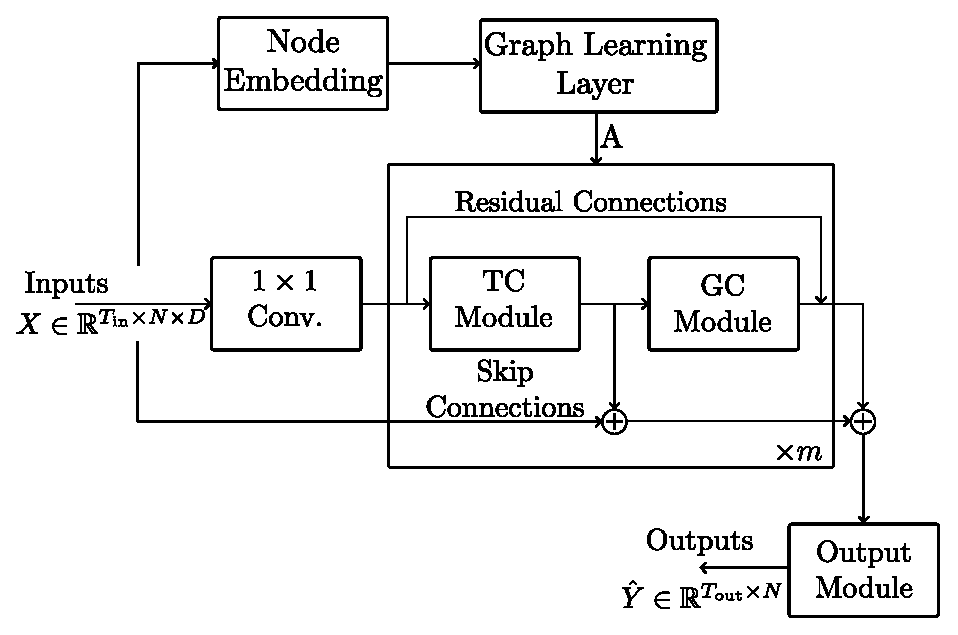
\includegraphics[width=0.48\textwidth]{./figures/gnn_architecture_v1.eps}
  \caption{The architecture of the spatio-temporal graph neural network.} 
  \label{fig:gnn_architecture}
\end{figure}
%

\subsection{Baseline Forecasting Methods for Comparison}
\label{ssec:multi_ts}
%
We establish baselines to compare and contrast MTGNN with by measuring the performance of four other 
prominent methods used to process multivariate time series data. One is the classical autoregressive (AR) model, 
while the rest are neural-network-based methods: autoregressive-multilayer perception (VAR-MLP), 
recurrent neural network (RNN-GRU) and temporal convolutional network (TCN).


An autoregressive model assumes that the current value of a time series is a function of its past values. In other words, AR model is when a value from a time series is regressed on previous values from that same time series. In this regression model, the response variable in the previous time period has become the predictor and the errors have usual assumptions about errors in a simple linear regression model. The order of an autoregression is the number of immediately preceding values in the series that are used to predict the value at the present time ~\citep{penn}. 

The vector autoregressive (VAR) model is a well-known statistical model used to capture linear interdependencies among multiple time series. It has been widely applied in econometrics for modeling and forecasting systems where multiple variables influence each other over time ~\citep{lutkepohl2005new}. However, VAR models assume linear relationships, which can be limiting in cases where the underlying data exhibits complex, nonlinear dynamics. To address this limitation, the VAR-MLP model incorporates the MLP, a type of artificial neural network known for its ability to learn and approximate nonlinear functions. By combining VAR with MLP, the VAR-MLP model leverages the strengths of both methods: it captures the linear interdependencies among multiple time series using VAR, while the MLP component models the potential nonlinear relationships that VAR cannot. This hybrid approach allows for more accurate modeling and forecasting in systems where both linear and nonlinear interactions are significant, as demonstrated in empirical studies across various domains, including finance and economics ~\citep{zhang2003time, zivot2006modeling}. The flexibility of VAR-MLP makes it particularly effective in complex systems where traditional linear models may fall short, thus providing a comprehensive framework for time series analysis. 

RNNs are a class of neural networks designed to handle sequential data by maintaining a hidden state that captures information from previous inputs ~\citep{hochreiter1997long}. However, RNNs suffer from issues like vanishing gradients, which limit their ability to learn long-term dependencies. To address this, the Gated Recurrent Unit (GRU) was introduced as an improved variant of the RNN ~\citep{cho2014learning}. The GRU uses gating mechanisms—namely, an update gate and a reset gate—to control the flow of information, making it more efficient at capturing dependencies over longer sequences while reducing the complexity ~\citep{chung2014empirical}. This innovation allows GRUs to perform better than traditional RNNs in various sequential modeling tasks by mitigating the vanishing gradient problem and simplifying the model structure.

TCNs are a type of neural network architecture designed for sequence modeling tasks, offering an alternative to Recurrent Neural Networks (RNNs) and Long Short-Term Memory (LSTM) networks. TCNs leverage the strengths of convolutional neural networks (CNNs) by using 1D convolutions to process sequential data, enabling them to capture temporal dependencies over long sequences efficiently. Unlike RNNs, TCNs do not suffer from issues like vanishing gradients and can handle much longer input sequences due to their ability to employ dilated convolutions, which exponentially increase the receptive field of the network without a corresponding increase in computational cost ~\citep{bai2018empirical}. Additionally, TCNs use causal convolutions, ensuring that the output at any time step is only influenced by past inputs, maintaining the temporal order of the data ~\citep{oord2016wavenet}. This structure allows TCNs to outperform traditional RNNs and LSTMs in various tasks, such as time series forecasting, due to their stable training dynamics and ability to capture long-range dependencies ~\citep{bai2018empirical}.

\subsection{Evaluation metrics}
\label{ssec:metric}

The metrics we used for measuring the performance of various algorithms are relative squared error (RSE), root mean squared error 
(RMSE), mean absolute error (MAE) and mean absolute percentage error (MAPE). The mathematical expressions for 
these metrics are given below.
%
\begin{align}
    \operatorname{RSE} &= \frac{\sum_{i=1}^N \left(y_i - \hat{y}_i\right)^2}{\sum_{i=1}^N \left(y_i - \bar{y}\right)^2}, \\
    \operatorname{RMSE} &= \sqrt{\frac{\sum_{i=1}^N \left(y_i - \hat{y}_i\right)^2}{N}}, \\
    \operatorname{MAE} &= \frac{\sum_{i=1}^N \abs{y_i - \hat{y}_i}}{N}, \\
    \operatorname{MAPE} &= \frac{1}{N}\sum_{i=1}^N \abs{\frac{y_i - \hat{y}_i}{y_i}},
\end{align}
%
where $\hat{y}_i$ is the value predicted by the algorithm for observation $i$ (out of $N$ observations), $y_i$ is 
the actual value, and $\bar{y}$ is the average of all target values. For a perfect fit, each of these 
measures would assume the value $0$. Hence, they range from $0$ to $\infty$ with $0$ corresponding to 
the ideal.
